\subsubsection{DTO (Data Transfer Objects)}

\subsubsubsection{Introduzione}
\par Questa sezione descrive le classi che rappresentano \glossario{DTO} (Data Transfer Objects), ossia design pattern utilizzati per il tasferimento dei dati tra gli strati dell'applicazione. I DTO sono dei contenitori semplici e privi di logica di business, progettati per aggregare dati e facilitare la comunicazione tra i componenti del sistema.

\subsubsubsection{ResponseStatusEnum} \label{ResponseStatusEnum} 
\begin{figure}[H]
    \centering
    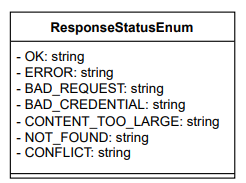
\includegraphics[width=0.4\textwidth]{assets/Backend/response_status_enum.png}
    \caption{Diagramma della classe ResponseStatusEnum}
\end{figure}
\par ResponseStatusEnum è un'enumerazione che rappresenta i possibili stati di risposta del sistema. Le coppie chiave-valore sono basate sui codici di stato HTTP.

\subsubsubsection{ResponseDto} \label{ResponseDto}
\begin{figure}[H]
    \centering
    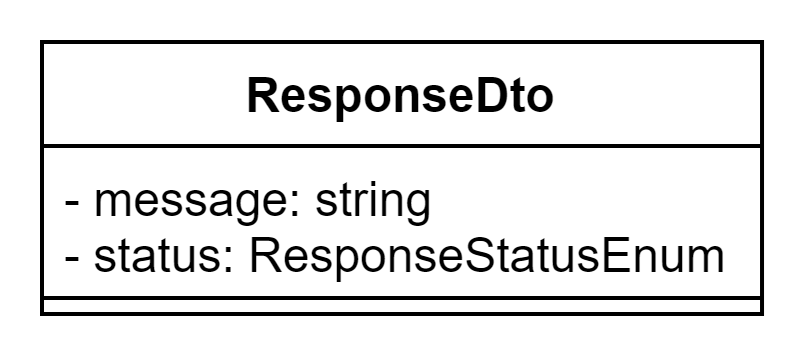
\includegraphics[width=0.4\textwidth]{assets/Backend/response_dto.png}
    \caption{Diagramma della classe ResponseDto}
  \end{figure}
\par ResponseDto è un DTO utilizzato per rappresentare una risposta standardizzata del sistema. La classe contiene un messaggio esplicativo e un'istanza di ResponseStatusEnum.

\subsubsubsection{StringDataResponseDto} \label{StringDataResponseDto}
\begin{figure}[H]
    \centering
    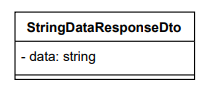
\includegraphics[width=0.4\textwidth]{assets/Backend/string_data_response_dto.png}
    \caption{Diagramma della classe StringDataResponseDto}
  \end{figure}
\par StringDataResponseDto è un DTO utilizzato per rappresentare una risposta del sistema che include dati testuali. La classe estende ResponseDto.

\subsubsubsection{AuthResponseDto} \label{AuthResponseDto}
\begin{figure}[H]
    \centering
    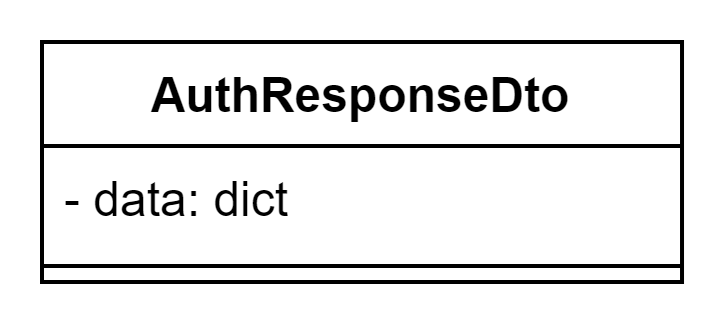
\includegraphics[width=0.4\textwidth]{assets/Backend/auth_response_dto.png}
    \caption{Diagramma della classe AuthResponseDto}
  \end{figure}
\par AuthResponseDto è un DTO utilizzato per rappresentare la risposta del sistema a una richiesta di autenticazione. La classe estende ResponseDto.

\subsubsubsection{DictionaryResponseDto} \label{DictionaryResponseDto}
\begin{figure}[H]
    \centering
    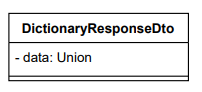
\includegraphics[width=0.5\textwidth]{assets/Backend/dictionary_response_dto.png}
    \caption{Diagramma della classe DictionaryResponseDto}
  \end{figure}
\par DictionaryResponseDto è un DTO utilizzato per rappresentare una risposta del sistema che include dati relativi a uno specifico dizionario. Le informazioni possono includere le caratteristiche di un dizionario o un'anteprima del suo contenuto. La classe estende ResponseDto.

\subsubsubsection{DictionariesResponseDto} \label{DictionariesResponseDto}
\begin{figure}[H]
    \centering
    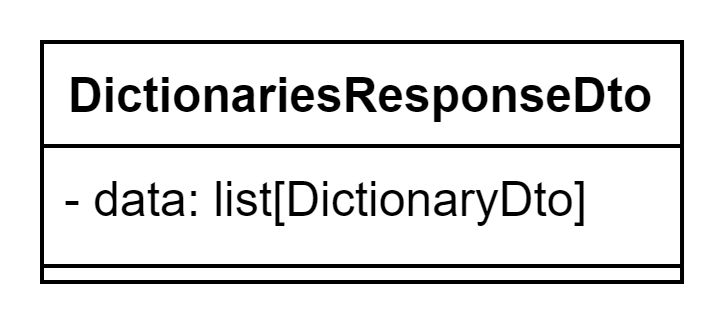
\includegraphics[width=0.4\textwidth]{assets/Backend/dictionaries_response_dto.png}
    \caption{Diagramma della classe DictionariesResponseDto}
  \end{figure}
\par DictionariesResponseDto è un DTO utilizzato per rappresentare una risposta del sistema contenente una lista di dizionari con le loro caratteristiche specifiche. La classe estende ResponseDto.

\subsubsubsection{PromptResponseDto} \label{PromptResponseDto}
\begin{figure}[H]
    \centering
    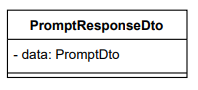
\includegraphics[width=0.4\textwidth]{assets/Backend/prompt_response_dto.png}
    \caption{Diagramma della classe PromptResponseDto}
  \end{figure}
\par PromptResponseDto è un DTO utilizzato per rappresentare una risposta del sistema che include dati relativi a un \glossario{prompt}. La classe estende ResponseDto.

\subsubsubsection{LoginDto} \label{LoginDto}
\begin{figure}[H]
    \centering
    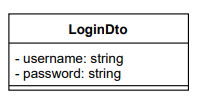
\includegraphics[width=0.4\textwidth]{assets/Backend/login_dto.png}
    \caption{Diagramma della classe LoginDto}
  \end{figure}
\par LoginDto è un DTO utilizzato per gestire i dati di autenticazione durante il processo di login. Le credenziali di accesso includono lo username e la password.

\subsubsubsection{AdminDto} \label{AdminDto}
\begin{figure}[H]
    \centering
    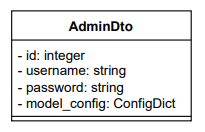
\includegraphics[width=0.4\textwidth]{assets/Backend/admin_dto.png}
    \caption{Diagramma della classe AdminDto}
  \end{figure}
\par AdminDto è un DTO utilizzato per modellare i dati degli utenti con privilegi di amministratore nel sistema. Oltre a username e password, il DTO contiene un identificatore numerico univoco.

\subsubsubsection{DictionaryDto} \label{DictionaryDto}
\begin{figure}[H]
    \centering
    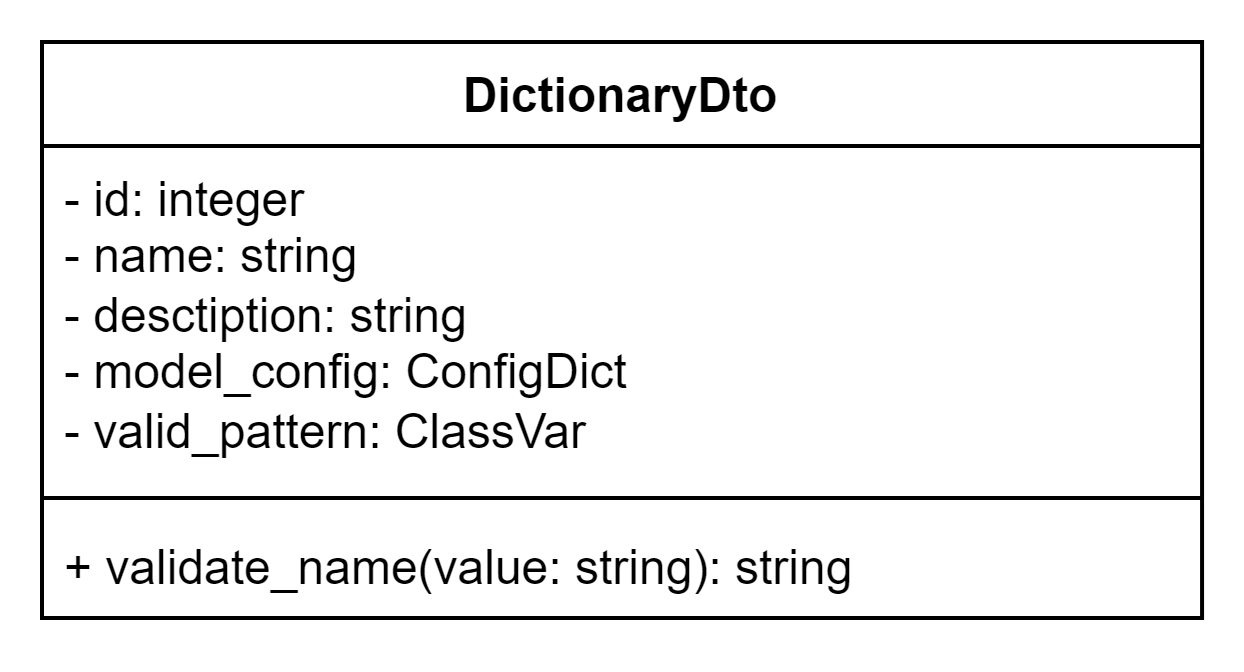
\includegraphics[width=0.5\textwidth]{assets/Backend/dictionary_dto.png}
    \caption{Diagramma della classe DictionaryDto}
\end{figure}
\par DictionaryDto è un DTO utilizzato per modellare le informazioni relative a un dizionario, inclusi il nome e la descrizione. La classe contiene un metodo di validazione per il campo "name".

\subsubsubsection{DictionaryPreviewDto} \label{DictionaryPreviewDto}
\begin{figure}[H]
    \centering
    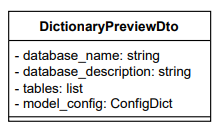
\includegraphics[width=0.4\textwidth]{assets/Backend/dictionary_preview_dto.png}
    \caption{Diagramma della classe DictionaryPreviewDto}
  \end{figure}
\par DictionaryPreviewDto è un DTO utilizzato per fornire una panoramica di un \glossario{dizionario dati}. L'anteprima include il nome e la descrizione del \glossario{database}, insieme a una lista di tabelle con le loro informazioni.

\subsubsubsection{TableDto} \label{TableDto}
\begin{figure}[H]
    \centering
    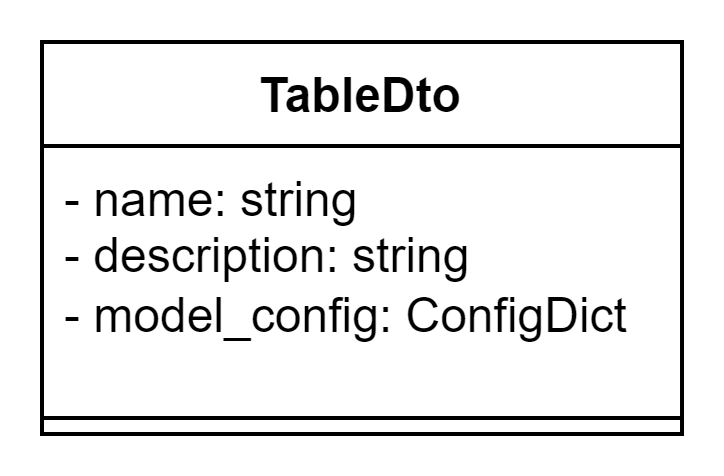
\includegraphics[width=0.4\textwidth]{assets/Backend/table_dto.png}
    \caption{Diagramma della classe TableDto}
  \end{figure}
\par TableDto è un DTO utilizzato per rappresentare i dati relativi a una tabella contenuta all'interno di un \glossario{dizionario dati}. Ogni tabella è corredata da un nome e da una descrizione.

\subsubsubsection{PromptDto} \label{PromptDto}
\begin{figure}[H]
    \centering
    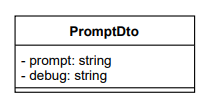
\includegraphics[width=0.4\textwidth]{assets/Backend/prompt_dto.png}
    \caption{Diagramma della classe PromptDto}
\end{figure}
\par PromptDto è un DTO utilizzato per modellare il \glossario{prompt} generato dal sistema. La classe contiene due campi di tipo stringa: il testo del prompt e le informazioni di \glossario{debug} relative ad esso.